
\subsection{Performance Formula}
\label{sub-sec:formula}
\todo{perf = want and can} \newline

\subsection{PRAE Model}
\label{sub-sec:prae}


Each person has it's own personality and from a psychological point of view there are different indicator types. One of these indicators are the Myers-Brigs indicator \cite{myers} (based on the research of C. Jung) and offer 8 personality traits that result in 16 personality types. This traits are:
\begin{itemize}
\item extroversion(E) / introversion (I)
\item sensing (S) / intuition(N)
\item thinking (T) / feeling (F) 
\item judgement (J) / perception (P)
\end{itemize}
Each person has one of the two traits from each of the categories above, and the different combination result in 16 possible personalities. Their interpretations can be found at \cite{mbf}.

Although the Myers-Brigs indicator was intended to be used by people with no qualifications in psychology, in practice it has proven very difficult for managers to identify the correct traits of their employees without using extensive tests. A simpler model was developed in order to help managers in interacting with their employees based on their personality. 

\begin{figure}[h]
\centering
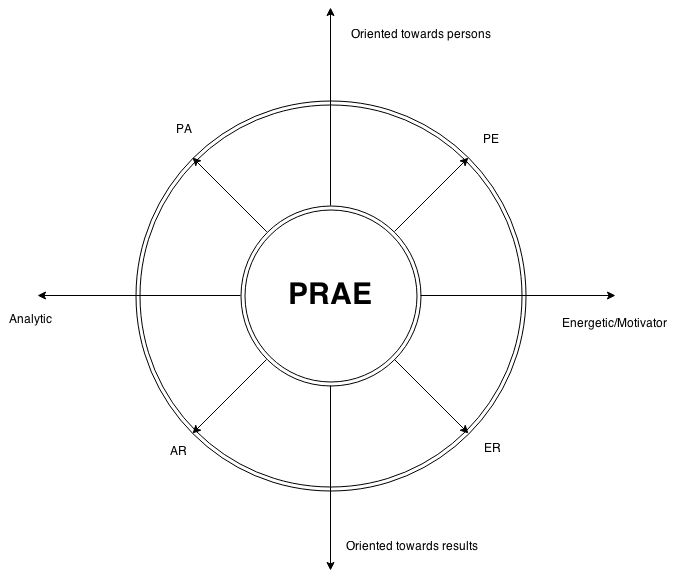
\includegraphics[width=0.8\textwidth]{img/prae.png}
\caption{PRAE personality model}
\label{fig:prae}
\end{figure}

The \textbf{PRAE} model is based on 4 traits, and as the name suggest the traits are:
\begin{itemize}
\item Person oriented
\item Result oriented
\item Analytical
\item Energetic(motivator)
\end{itemize}

Based on the PRAE model, each parson has a dominant trait that he uses in most situations and is usually the way that a person feels most comfortable to act as. A person also has a secondary trait that he usually uses in unusual/under-pressure situations. At the opposite end there is the adverse trait that hints the behaviour that a person is least comfortable to use.



In \ref{fig:prae} the vertical axis (P-R) is called \textit{Scope of action} and the horizontal axis (A-E) is called the \textit{Style of action}. As \ref{fig:prae} hints(although not impossible) the dominant and secondary traits are usually found on different axis. 

Although there are a lot of questionnaires to determine the PRAE model for each person, the dominant and secondary trait can be easily determined by the language that a person uses. In \ref{table:prae} can be found a description of the strong points, weak points and language indicator according to each PRAE trait.

\begin{table}[h]
  \centering
  \caption{Prae dreakdown detalis}
  \setlength\tabcolsep{3.8pt}
  \setlength\extrarowheight{1pt}
    \begin{tabular}{ | p{0.11\textwidth} | p{0.3\textwidth} | p{0.3\textwidth} | p{0.29\textwidth} |}
    \hline
    Trait & Strong points & Week Points & Language Indicators \\ \hline
    
    Person oriented 
     &
      \begin{itemize}
      \item he cares
      \item tactful
      \item motivating
      \item peacemaker, pacifist
      \item looks for cooperation and consensus
      \item tries to involve all the parties
      \end{itemize}
     & 
      \begin{itemize}
      \item easily offend
      \item very emotive
      \item listens to "what the others say"
      \item constantly looking for approval
      \item wishes to please everybody
      \item procrastination in making decisions
      \end{itemize}
     & 
      \begin{itemize}
      \item words like \textit{we, together}
      \item protective vocabulary
      \item do not get straight to the point
      \item spoiled behaviour
      \end{itemize}
     \\ \hline
    Results oriented
     &
      \begin{itemize}
       \item focuses on end result
       \item competitive
       \item honest and straight forward
       \item risk takers
       \item work well under pressure
      \end{itemize}
     &
      \begin{itemize}
       \item do not have patience with people
       \item sometimes sarcastic and insensible
       \item anti rules or processes
       \item individualists
       \item think in black or white
       \item become frustrated by persons who are afraid of risks
      \end{itemize}
     & 
     \begin{itemize}
      \item phrases like: I want
      \item Asks for facts and numbers
      \item Asks \textit {What's in it for me}
      \item Short time spent talking about \textit {how to do it}
     \end{itemize}
     \\ \hline
    Analytical
     &
      \begin{itemize}
       \item precise
       \item looks for proof and validation
       \item plans everything in a step by step way
       \item focused on facts and numbers
       \item sets high standards
      \end{itemize}
     &
      \begin{itemize}
       \item favours processes over results or relationships
       \item tendency to pessimism
       \item critic
       \item suffers from \textit{Paralysis by Analysis}
       \item can portrait intellectual arrogance.
      \end{itemize}
     &
      \begin{itemize}
       \item words like: must and depends
       \item asks for all the details
       \item gets irritated if interrupted
       \item gets frustrated when told how to do his work
      \end{itemize}
     \\ \hline
    Energetic 
     &
      \begin{itemize}
       \item enthusiast
       \item likes variety
       \item creates a friendly environment
       \item persuasive 
       \item spontaneous
       \item likes to have fun
       \item optimist
      \end{itemize}
     &
     \begin{itemize}
      \item impulsive
      \item thinks out loud
      \item disorganized, superficial
      \item easily bored
      \item skips analysis
      \item looks for attention and recognition
     \end{itemize}
     & 
      \begin{itemize}
       \item excessive use of words hinting his person: Me, I 
       \item makes himself the center of attention
       \item reacts positively to phrases like: You can, You will
      \end{itemize}
     \\ \hline
    \end{tabular}
    \label{table:prae}
\end{table}
\FloatBarrier

In the IT industry I observed that in 50\% of cases the combination between dominant and secondary trait is formed from \textit{Analytical} and \textit{Results}. This kind of persons are real assets to a company that is already established and focusses more on quality and not on delivering new features using short deadlines. For continuing to add new value to a product a person that has a mix made from \textit{Results} and \textit{Energetic} person is needed. The biggest drawback I observed for this mix is that this kind of person easily looses it's focus if something new needs to be implement, thus starting to work on new things without analysing all the possible use-cases and delivering software that works only on positive scenarios.
\subsection{RACI Matrix}
\label{sub-sec:raci}
\todo{RACI} \newline

\subsection{FAC Model}
\label{sub-sec:fac}
\todo{FAC feedback} \newline